\subsection{Vinculación del lector}

La vinculación del lector se realiza a través de la generación de dos códigos de barras que funcionan a modo de tokens. Al generarse los dos códigos; estos quedan asociados al identificador del usuario.

El flujo de la vinculación de un lector con la cuenta de un usuario es el siguiente:

\begin{figure}[H]
    \centering
    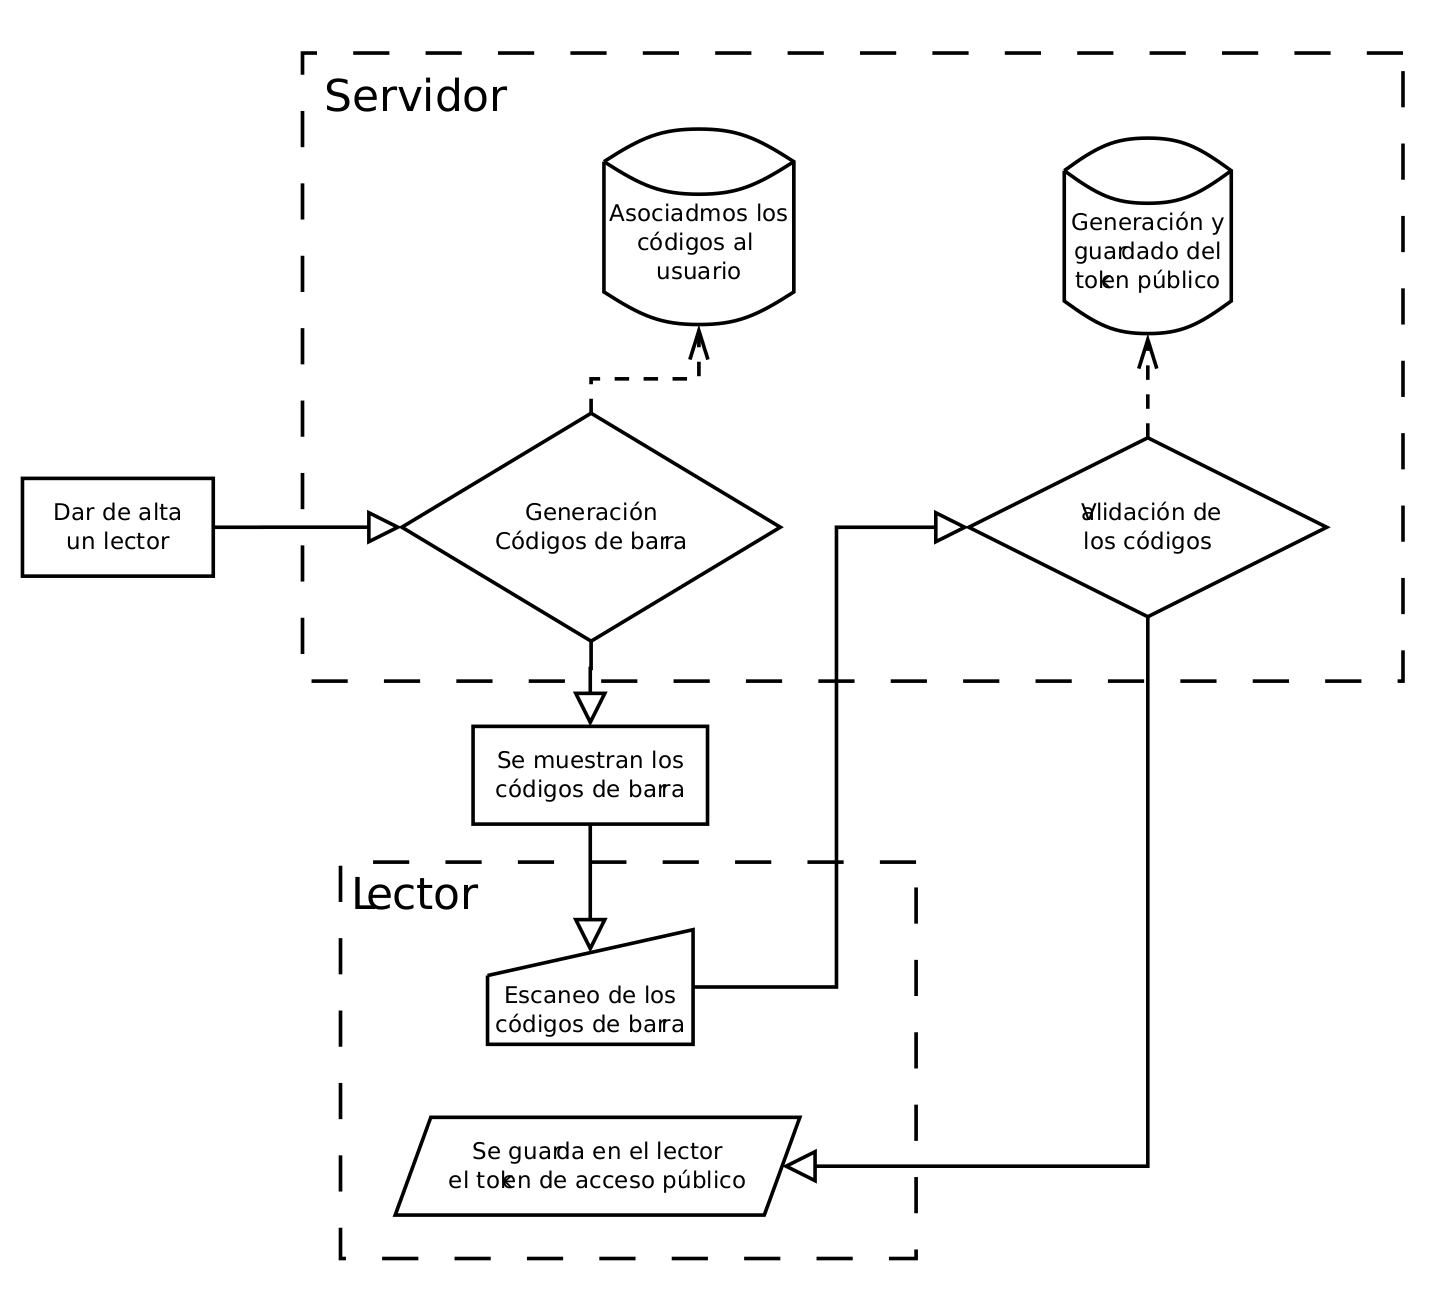
\includegraphics[keepaspectratio,width=0.9\textwidth]{flujo-vinculacion-lector.png}
    \caption{Flujo de la vinculación de un lector}\label{fig:flujo-vinculacion-lector}
\end{figure}

El servidor se encarga de generar y verificar los códigos de barra, asociando si la vinculación es correcta una clave de acceso pública al lector. Así, en las siguientes peticiones (añadir productos, sacar...) el lector deberá enviar junto con la información del producto, la clave pública.